% ======================================================================
% fig_lr_criterion -- standalone build of a figure that main.tex also draws inline.
% ----------------------------------------------------------------------
% The tikzpicture below is copied VERBATIM from main.tex, so this file and
% the inline version render identically. Build with:
%     pdflatex fig_lr_criterion.tex
% The standalone class crops the PDF to the picture's bounding box, so no
% trim/clip is ever needed in the paper.
%
% Fonts: the picture inherits times/helvet, so every glyph is Type 1 and
% embedded by pdflatex. Nothing is rasterised, so DPI does not apply.
% ======================================================================
\documentclass[border=2pt]{standalone}

\usepackage{times}
\usepackage{helvet}
\usepackage{courier}
\usepackage{amsmath}
\usepackage{amssymb}
\usepackage{xcolor}
\usepackage{pifont}
\usepackage{tikz}
\usetikzlibrary{arrows.meta,positioning}

%% ======================================================================
%% preamble-figures.tex
%% ----------------------------------------------------------------------
%% Every definition the figures need, kept identical to main.tex's preamble.
%% Shared by the standalone builds in this folder; main.tex carries its own
%% copy so that the submitted source stays a single .tex file.
%% ======================================================================

\providecommand{\method}{\textsc{ESV}}

%% --- comparison-table glyphs (fig_trap uses \yes / \no) ---------------
\definecolor{okgreen}{RGB}{0,122,87}
\definecolor{okred}{RGB}{176,42,32}
\providecommand{\yes}{\textcolor{okgreen}{\ding{51}}}
\providecommand{\no}{\textcolor{okred}{\ding{55}}}
\providecommand{\na}{\textcolor{black!45}{--}}

%% --- figure fills, shaded by what each step costs ---------------------
\definecolor{cshared}{RGB}{226,226,226}
\definecolor{ccode}{RGB}{205,228,243}
\definecolor{ccall}{RGB}{252,230,192}
\definecolor{ccallb}{RGB}{191,118,0}
\definecolor{cout}{RGB}{206,238,227}
\definecolor{ctrap}{RGB}{250,222,218}

%% --- plot colours and markers -----------------------------------------
%% Marker shapes are core TikZ nodes, so every glyph is vector and uses the
%% document's Type 1 text fonts: no Type 3 subsets, no raster, nothing to crop.
\definecolor{pblue}{RGB}{31,97,160}
\definecolor{pgreen}{RGB}{0,122,87}
\definecolor{pgrey}{RGB}{95,95,95}
\providecommand{\mkopensq}[2]{\node[draw=#2,fill=white,line width=.6pt,rectangle,inner sep=1.5pt] at #1 {};}
\providecommand{\mkfillsq}[2]{\node[draw=#2,fill=#2,rectangle,inner sep=1.5pt] at #1 {};}
\providecommand{\mkopenci}[2]{\node[draw=#2,fill=white,line width=.6pt,circle,inner sep=1.5pt] at #1 {};}
\providecommand{\mkfillci}[2]{\node[draw=#2,fill=#2,circle,inner sep=1.5pt] at #1 {};}
%% #1 x, #2 centre, #3 half-width of the interval, #4 colour (needs x=1cm)
\providecommand{\ebar}[4]{%
  \draw[#4,line width=.5pt] (#1,{#2-#3}) -- (#1,{#2+#3});
  \draw[#4,line width=.5pt] ({#1-0.055},{#2-#3}) -- ({#1+0.055},{#2-#3});
  \draw[#4,line width=.5pt] ({#1-0.055},{#2+#3}) -- ({#1+0.055},{#2+#3});}

%% --- \cost is used inside the three schematic figures -----------------
\providecommand{\cost}{\scriptsize}


\begin{document}
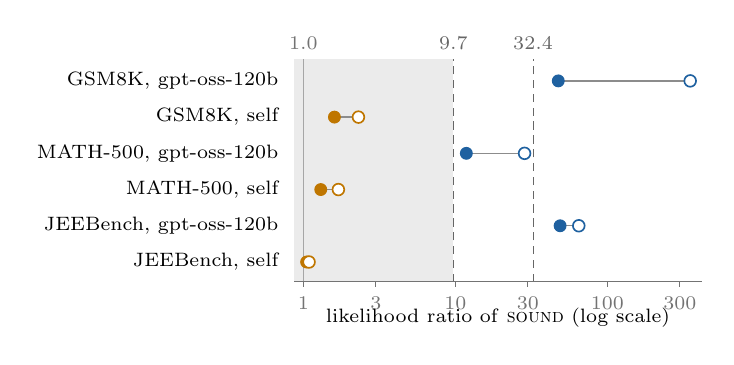
\begin{tikzpicture}[x=1.93cm, y=0.46cm, font=\footnotesize]
%% no untied vote can be overturned left of the 2--1--1 bar
\fill[black!8] (-0.06,0.45) rectangle (0.987,6.60);
%% Eq. (2) bars for the vote splits four samples allow
\draw[black!35] (0,0.45) -- (0,6.60)
  node[anchor=south, font=\scriptsize, black!55] {$1.0$};
\draw[black!60, densely dashed] (0.987,0.45) -- (0.987,6.60)
  node[anchor=south, font=\scriptsize] {$9.7$};
\draw[black!60, densely dashed] (1.511,0.45) -- (1.511,6.60)
  node[anchor=south, font=\scriptsize] {$32.4$};
%% x axis, decade ticks
\draw[black!55] (-0.06,0.45) -- (2.62,0.45);
\foreach \x/\lab in {0/1, 0.477/3, 1/10, 1.477/30, 2/100, 2.477/300}
  \draw[black!55] (\x,0.45) -- (\x,0.30) node[below=0pt, font=\scriptsize] {$\lab$};
\node[font=\scriptsize] at (1.28,-0.55) {likelihood ratio of \textsc{sound} (log scale)};
%% rows: filled = Lambda_S, open = Lambda_S+F, joined
\newcommand{\lrrow}[4]{%
  \node[anchor=east, font=\scriptsize] at (-0.10,#1) {#2};
  \draw[black!45, line width=.5pt] (#3,#1) -- (#4,#1);}
\lrrow{6}{GSM8K, gpt-oss-120b}{1.677}{2.545}
  \mkfillci{(1.677,6)}{pblue}  \mkopenci{(2.545,6)}{pblue}
\lrrow{5}{GSM8K, self}{0.204}{0.362}
  \mkfillci{(0.204,5)}{ccallb} \mkopenci{(0.362,5)}{ccallb}
\lrrow{4}{MATH-500, gpt-oss-120b}{1.072}{1.455}
  \mkfillci{(1.072,4)}{pblue}  \mkopenci{(1.455,4)}{pblue}
\lrrow{3}{MATH-500, self}{0.114}{0.230}
  \mkfillci{(0.114,3)}{ccallb} \mkopenci{(0.230,3)}{ccallb}
\lrrow{2}{JEEBench, gpt-oss-120b}{1.689}{1.812}
  \mkfillci{(1.689,2)}{pblue}  \mkopenci{(1.812,2)}{pblue}
\lrrow{1}{JEEBench, self}{0.021}{0.037}
  \mkfillci{(0.021,1)}{ccallb} \mkopenci{(0.037,1)}{ccallb}
\end{tikzpicture}
\end{document}
